\section{Aufbau}
Der Versuch besteht prinzipiell aus drei Geräten. Dem Nadelimpulsgenerator, dem Schaltkreis aus Kondensator $C$, Widerstand $R$ und Spule $L$, und dem Oszilloskop. 
In den folgenden Abbildungen zu beachten ist, dass auf drei verschiedene Widerstände zugegriffen werden kann. Es sind zwei unterschiedlich große und ein verstellbarer Widerstand gegeben. 
\subsection{Zeitabhängigkeit der Amplitude (a)}

Die Messung des ersten Versuchteils erfolgen über folgende Schaltung:
\begin{figure}[H]
  \centering
  \includegraphics[height=5cm]{Aufbau/Grafiken/a.pdf}
  \caption{Aufbau zu (a), \cite{1}.}
  \label{fig:a}
\end{figure}

\subsection{Dämpfungswiderstand}

Der Dämpfungswiderstand wird über die abgebildete Schaltung \ref{fig:b} bestimmt.
\begin{figure}[H]
  \centering
  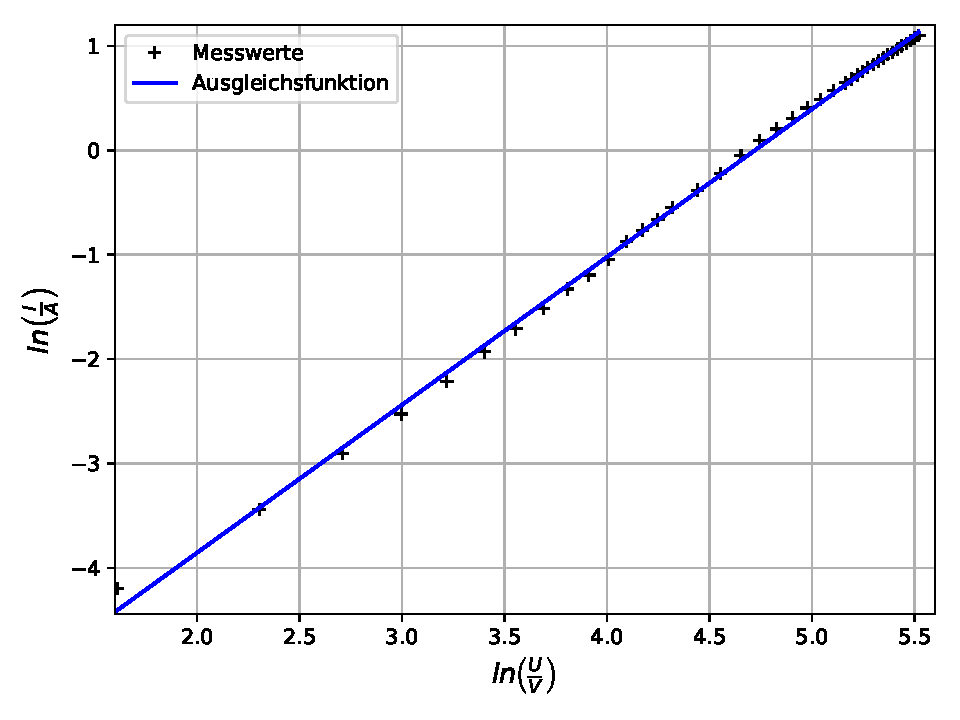
\includegraphics[height=5cm]{Aufbau/Grafiken/b.pdf}
  \caption{Aufbau zu (b), \cite{1}.}
  \label{fig:b}
\end{figure}
\newpage
\subsection{Frequenzabhängigkeit der Kondensatorspannung}

Der Aufbau für den dritten Teil des Versuches, der Bestimmung der Frequenzabhängigkeit der Kondensatorspannung, ist in Abbildung \ref{fig:c} abgebildet.
\begin{figure}[H]
  \centering
  \includegraphics[height=5cm]{Aufbau/Grafiken/c.pdf}
  \caption{Aufbau zu (c), \cite{1}.}
  \label{fig:c}
\end{figure}

\subsection{Frequenzabhängigkeit der Phasenverschiebung}

Zur Bestimmung der Frequenzabhängigkeit der Phasenverschiebung wird der Aufbau aus Abbildung \ref{fig:d} verwendet.
\begin{figure}[H]
  \centering
  \includegraphics[height=5cm]{Aufbau/Grafiken/d.pdf}
  \caption{Aufbau zu (d), \cite{1}.}
  \label{fig:d}
\end{figure}